\documentclass[11pt]{article}
\usepackage[margin=1in]{geometry}
\usepackage{amsmath}
\usepackage{graphicx}
\usepackage{hyperref}

\title{FFT Peak Interpolation: Quadratic vs.\ Quartic Fits,\\
and the Zero-at-Center / Worst-near-Quarter-Bin Bias Pattern}
\author{}
\date{}

\begin{document}
\maketitle

\section{The problem}

A tone sampled by an $N$-point FFT almost never lands exactly on a bin
center. Writing the true frequency as $k_0 + \delta$ bins, with
$\delta \in [-0.5, 0.5]$ the fractional offset from the nearest bin
$k_0$, the three complex DFT values around the peak are
\begin{equation}
  X_{-1} = X(k_0-1), \qquad X_0 = X(k_0), \qquad X_{+1} = X(k_0+1).
\end{equation}
The interpolation problem is: given only these three complex numbers,
estimate $\delta$ as accurately as possible.

\section{Approach 1: fit the complex spectrum directly (quartic)}

$X_{-1}, X_0, X_{+1}$ are complex, so one natural idea is to fit a
quadratic to the real parts $\operatorname{Re}X(k)$ and a second,
independent quadratic to the imaginary parts $\operatorname{Im}X(k)$,
each as a function of bin index $k$. With exactly three points, each
fit is an exact (Lagrange) interpolation, not a least-squares fit:
\begin{align}
  R(x) &= a_R x^2 + b_R x + c_R, \qquad R(-1)=\operatorname{Re}X_{-1},\;
         R(0)=\operatorname{Re}X_0,\; R(1)=\operatorname{Re}X_{+1},\\
  I(x) &= a_I x^2 + b_I x + c_I, \qquad I(-1)=\operatorname{Im}X_{-1},\;
         I(0)=\operatorname{Im}X_0,\; I(1)=\operatorname{Im}X_{+1}.
\end{align}
The power at any (non-integer) offset $x$ is then
\begin{equation}
  P(x) = R(x)^2 + I(x)^2,
\end{equation}
a product of two quadratics squared and summed -- a genuine
\textbf{4th-order polynomial (quartic) in $x$}. Finding its true
maximum means solving $P'(x)=0$, a cubic equation, not reading off a
single vertex formula the way a quadratic allows.

This is a legitimate way to pose the problem, but it has a structural
weakness: a 3-point exact fit has no information about how the
spectrum behaves \emph{beyond} those three points. Nothing forces
$R(x)$ or $I(x)$ to decay away from the peak, so the quartic
$P(x)$ is not guaranteed to be well-behaved (single-peaked) over the
interval -- it can have its true maximum land on the wrong side of
the measured peak entirely as $\delta$ moves away from zero.
Figure~\ref{fig:quartic-vs-quadratic} shows this numerically: bias
exceeding half a bin by $\delta=0.5$, far worse than simply not
correcting at all.

\section{Approach 2: fit the power directly (quadratic)}

The practical alternative sidesteps the complex-plane fit entirely and
interpolates the (always real, always non-negative) \textbf{power}
\begin{equation}
  y_1 = |X_{-1}|^2, \qquad y_2 = |X_0|^2, \qquad y_3 = |X_{+1}|^2
\end{equation}
with a single quadratic. Because $|X(k)|^2$ for a windowed single tone
has a smooth, unimodal mainlobe shape with no sign changes, a
quadratic is a far more honest local model of it than it is of the
oscillating, phase-dependent $\operatorname{Re}X(k)$ or
$\operatorname{Im}X(k)$ individually. The standard 3-point vertex
formula gives the fractional correction directly, no cubic to solve:
\begin{equation}
  \delta \;=\; \frac{1}{2}\,\frac{y_1 - y_3}{y_1 - 2y_2 + y_3}.
  \label{eq:linear-power}
\end{equation}
A linear-power fit like Eq.~\eqref{eq:linear-power} still assumes a
parabolic mainlobe shape that no real window (rectangular or Hann)
actually has. Fitting the quadratic to the \emph{logarithm} of the
power instead matches a windowed mainlobe's real shape far better:
\begin{equation}
  \delta \;=\; \frac{1}{2}\,\frac{\ln y_1 - \ln y_3}
                                  {\ln y_1 - 2\ln y_2 + \ln y_3}.
  \label{eq:log-power}
\end{equation}
This is also a reason the power-domain fit is better-posed than the
complex-plane one in the first place: $|X(k)|^2$ is (to good
approximation) \textbf{independent of the tone's arbitrary phase}
at the start of the capture window, while $\operatorname{Re}X(k)$ and
$\operatorname{Im}X(k)$ individually are not. Two captures of the
same tone at the same frequency but different starting phase give
identical $y_1,y_2,y_3$, but different $(R,I)$ triples -- so a fit
built directly on $R$ and $I$ is modeling something that depends on a
quantity ($\delta$ and the phase) the quadratic has no way to
separate.

\section{Why the bias is zero at the bin center}

Equation~\eqref{eq:log-power} makes one fact immediate: if the true
frequency sits exactly on a bin ($\delta=0$), the spectrum is
symmetric about $k_0$, so $y_1 = y_3$ exactly. The numerator
$\ln y_1 - \ln y_3$ is then exactly zero, giving $\delta_{\text{est}}=0$
with \textbf{no approximation involved} -- this holds regardless of
noise, window choice, or $N$, purely from the symmetry of the three
points being fit.

\section{Why the bias returns to zero at the bin boundary, and peaks near a quarter bin}

The same symmetry argument extends to $\delta = 0.5$ (a tone sitting
exactly between two bins): for a symmetric window, the spectrum is
symmetric about the midpoint between $k_0$ and $k_0+1$, so the
3-point log-power fit again returns zero bias at that exact point.
Between these two zeros, the bias is not zero -- it rises from 0,
peaks, and falls back to 0, and from symmetry considerations alone the
extremum is expected near the midpoint of the interval, i.e.\ around
$\delta \approx 0.25$. Figure~\ref{fig:bias-symmetry} confirms this
numerically for the shipped Hann-window, log-power estimator at
$N=2048$: zero bias at $\delta=0$ and $\delta=0.5$, and a peak bias of
about $0.016$ bins near $\delta \approx 0.29$ -- in close agreement
with real bench measurements of the same formula ($-0.078\,$Hz at the
mid-bin point, corresponding to the same $\sim\!0.016$-bin scale).

\begin{figure}[h]
  \centering
  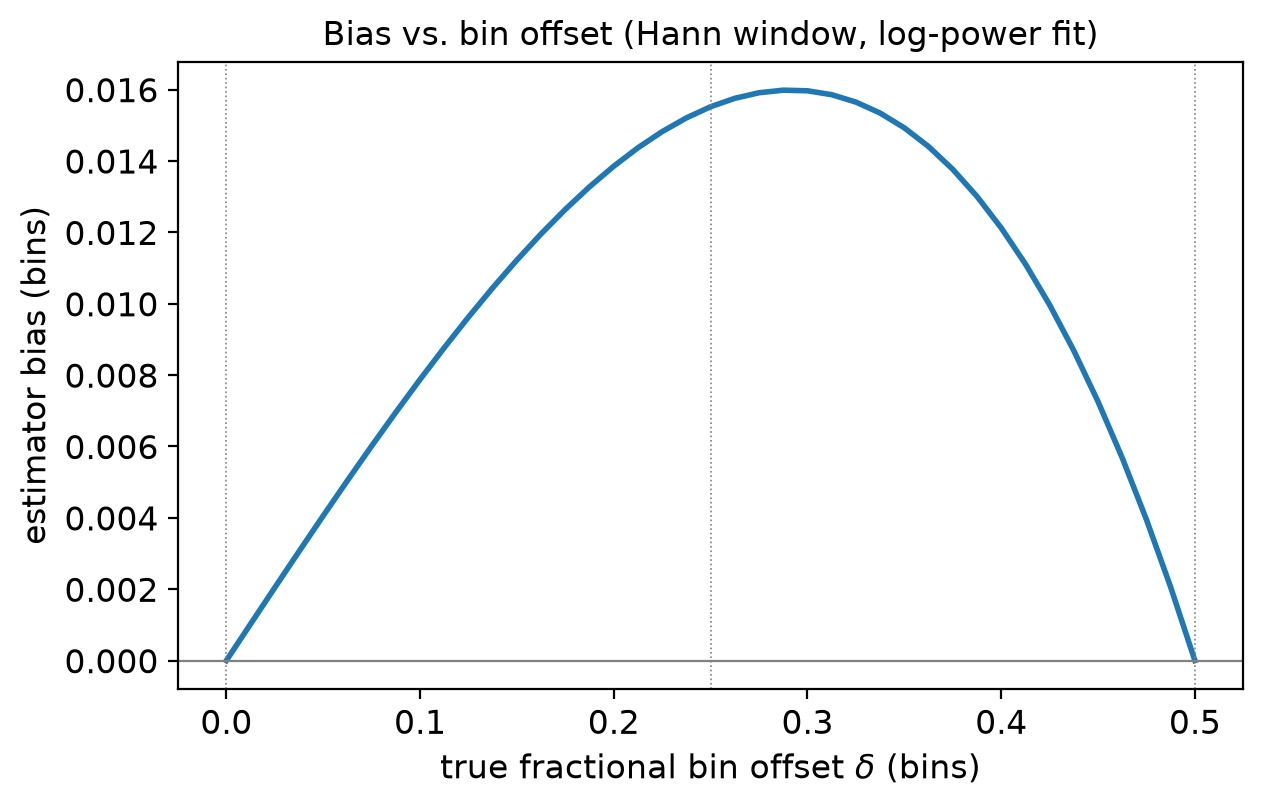
\includegraphics[width=0.75\textwidth]{fig_bias_symmetry.png}
  \caption{Bias of the Hann-windowed, log-power 3-point estimator as a
  function of the true fractional bin offset $\delta$. Bias is exactly
  zero at the bin center ($\delta=0$) and at the bin boundary
  ($\delta=0.5$), with the worst case near a quarter bin.}
  \label{fig:bias-symmetry}
\end{figure}

\begin{figure}[h]
  \centering
  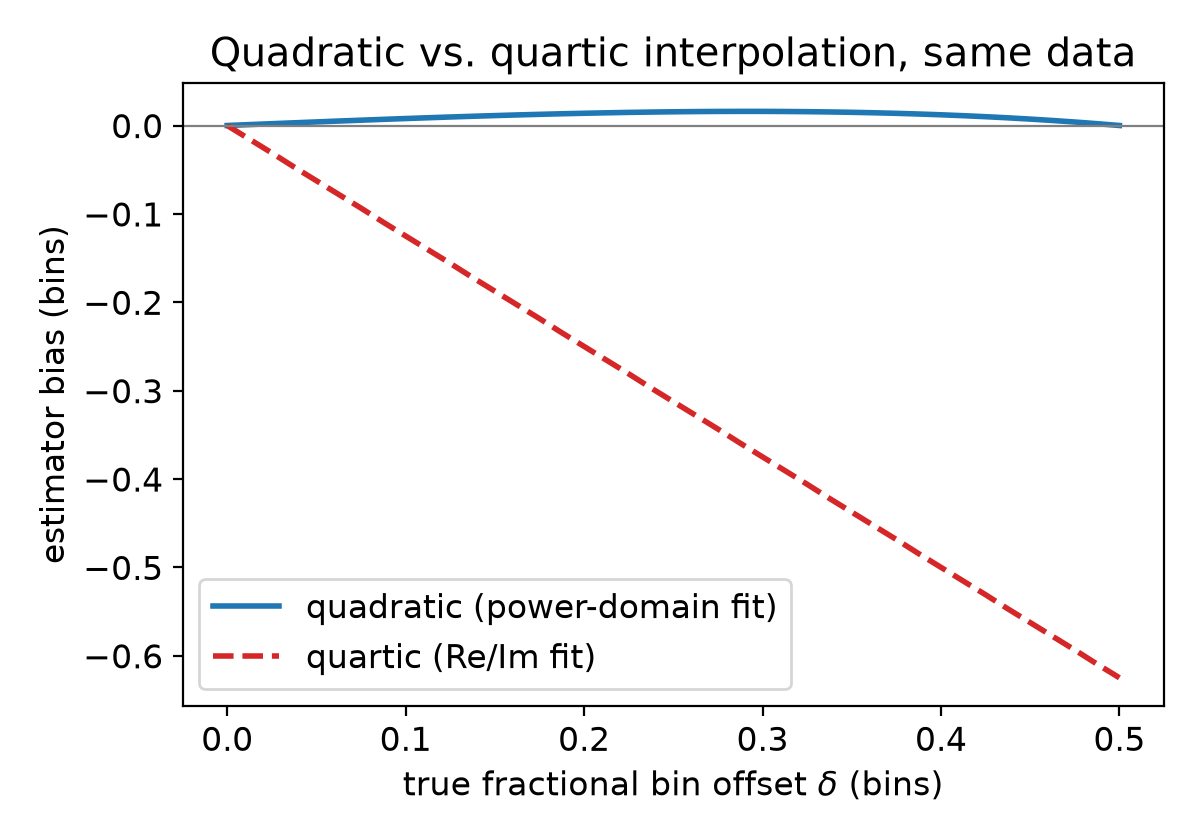
\includegraphics[width=0.75\textwidth]{fig_quartic_vs_quadratic.png}
  \caption{The power-domain quadratic fit (Eq.~\eqref{eq:log-power})
  compared against the quartic Re/Im fit from Section~2, on identical
  data. The quartic approach is not a refinement of the quadratic one
  -- it is substantially worse, because the unconstrained 3-point
  complex fit has no mechanism to stay well-behaved away from the
  measured bins.}
  \label{fig:quartic-vs-quadratic}
\end{figure}

\section{Summary}

\begin{itemize}
  \item Fitting quadratics to $\operatorname{Re}X(k)$ and
        $\operatorname{Im}X(k)$ separately and combining them produces
        a quartic power function whose true maximum requires solving
        a cubic -- and in practice is badly behaved away from the
        measured bins.
  \item Fitting a single quadratic (or log-quadratic) directly to the
        power $|X(k)|^2$ is both simpler and better motivated: power
        is phase-invariant and has a smooth, unimodal shape that a
        quadratic genuinely approximates well locally.
  \item The log-power fit's bias is exactly zero at the bin center and
        at the bin boundary, by symmetry of the three points being
        fit, with the worst case in between, near a quarter bin.
\end{itemize}

\section*{References}
\begin{itemize}
  \item E. Jacobsen, P. Kootsookos, ``Fast, Accurate Frequency
        Estimators,'' \emph{IEEE Signal Processing Magazine}, 2007.
  \item B. G. Quinn, ``Estimating Frequency by Interpolation Using
        Fourier Coefficients,'' \emph{IEEE Trans.\ Signal Processing},
        1994.
  \item F. J. Harris, ``On the Use of Windows for Harmonic Analysis
        with the Discrete Fourier Transform,'' \emph{Proc.\ IEEE},
        1978.
\end{itemize}

\end{document}
